\documentclass{article}
\usepackage[utf8]{inputenc}


\font\myfont=cmr12 at 25pt
%\title{\myfont Notes on Permanent Magnet Synchronous Machine (PMSM) Model %Predictive Control (MPC) and Operation Under Open Circuit Fault}
\font\hisfont=cmr12 at 15pt

\author{by \hisfont Hakan Sarac}
\date{}


\usepackage{float}
\usepackage{comment}
\usepackage{natbib}
\usepackage{graphicx}
\usepackage{indentfirst}
\usepackage{siunitx}
\usepackage{svg}
\usepackage{hyperref}
\usepackage{amsmath, bm}
\usepackage{graphicx} 
\usepackage{pstool}
\usepackage{listings}
\usepackage{natbib}
\usepackage{graphicx}
\usepackage{epstopdf}
\usepackage{tikz}
\usepackage[utf8]{inputenc}
\usepackage{pgfplots} 
\usepackage{pgfgantt}
\usepackage{pdflscape}
\usepackage[T1]{fontenc}
\usepackage{textcomp}
\usepackage{titlesec}
\usepackage{scrextend}
\usepackage[english]{babel}
\usepackage{blindtext}
\usepackage{movie15}
%\usepackage[colorlinks]{hyperref}

\pgfplotsset{compat=newest} 
\pgfplotsset{plot coordinates/math parser=false}
\lstloadlanguages{Matlab}%
\lstset{ 
	language=Matlab,                		% choose the language of the code
%	basicstyle=10pt,       				% the size of the fonts that are used for the code
	numbers=left,                  			% where to put the line-numbers
	numberstyle=\footnotesize,      		% the size of the fonts that are used for the line-numbers
	stepnumber=1,                   			% the step between two line-numbers. If it's 1 each line will be numbered
	numbersep=5pt,                  		% how far the line-numbers are from the code
%	backgroundcolor=\color{white},  	% choose the background color. You must add \usepackage{color}
	showspaces=false,               		% show spaces adding particular underscores
	showstringspaces=false,         		% underline spaces within strings
	showtabs=false,                 			% show tabs within strings adding particular underscores
%	frame=single,	                			% adds a frame around the code
%	tabsize=2,                				% sets default tabsize to 2 spaces
%	captionpos=b,                   			% sets the caption-position to bottom
	breaklines=true,                			% sets automatic line breaking
	breakatwhitespace=false,        		% sets if automatic breaks should only happen at whitespace
	escapeinside={\%*}{*)}          		% if you want to add a comment within your code
}

\addtolength{\oddsidemargin}{-.875in}
\addtolength{\evensidemargin}{-.875in}
\addtolength{\textwidth}{1.75in}
\addtolength{\topmargin}{-.875in}
\addtolength{\textheight}{1.75in}

\setcounter{secnumdepth}{4}

\titleformat{\paragraph}
{\normalfont\normalsize\bfseries}{\theparagraph}{1em}{}
\titlespacing*{\paragraph}
{0pt}{3.25ex plus 1ex minus .2ex}{1.5ex plus .2ex}


\begin{document}
\title{\line(1,0){250}\\\myfont Embedded Environment Visualizer Library Handbook \\\line(1,0){250}}
\maketitle
\newpage
\tableofcontents
\newpage


\section{Introduction}


This document explains how to use the Embedded Environment Visualizer Library (EEVL). EEVL consists of three parts: two matlab routines and a library. These parts are called:
\begin{itemize}
	\item \href{https://github.com/hakansrc/fault_tolerant_drives/blob/master/Software/MultipleDataPlot/DataReceiver.m}{DataReceiver.m}
	\item \href{https://github.com/hakansrc/fault_tolerant_drives/blob/master/Software/MultipleDataPlot/RawDataHandler.m}{RawDataHandler.m}
	\item \href{https://github.com/hakansrc/fault_tolerant_drives/tree/master/Software/MultipleDataPlot/MultipleFloatDataSender}{MultipleFloatDataSender library}
\end{itemize}

Each of these items are explained in their relevant section.
\newline
The aim of this library is to be able to collect, visualize and save data from an embedded environment, which is most of the time a trouble. 



\section{Matlab Routines} 
\subsection{\href{https://github.com/hakansrc/fault_tolerant_drives/blob/master/Software/MultipleDataPlot/DataReceiver.m}{DataReceiver.m}} 

This routine is the main routine that collects, saves, plots the received data on the computer. 
\subsubsection{Options}
\label{subsubsection:Options}
This routine has several options, which are:
\begin{itemize}
	\item \textbf{EnableSaving :} This enables/disables the saving of the received data. The received data is tagged with date and hour information.
	\item \textbf{ProcessRawDataThresholdInBytes :} When this routine received \textbf{ProcessRawDataThresholdInBytes} bytes of data, the received data is processed plotted/saved.
	\item \textbf{EnablePlotting :} This enables/disables the plotting of the received data. The received data is being plotted with time axis. 
	\item \textbf{DataSampleRate (Hz):} This variable is used for determining the time axis of the plotting. It should match the data sending rate of the DSP.
	\item \textbf{TheSerialChannelDevice :} The serial channel port seen by the computer is stated in this variable. The port value can be determined from the device manager. For the example given in Figure \ref{fig:DeviceManager}, TheSerialChannelDevice should be set as 'COM5'.
\end{itemize}

\subsection{\href{https://github.com/hakansrc/fault_tolerant_drives/blob/master/Software/MultipleDataPlot/RawDataHandler.m}{RawDataHandler.m}}
The saved data by \href{https://github.com/hakansrc/fault_tolerant_drives/blob/master/Software/MultipleDataPlot/DataReceiver.m}{DataReceiver.m} routine can be handled using this routine.



\begin{figure}[H]
	\centering
	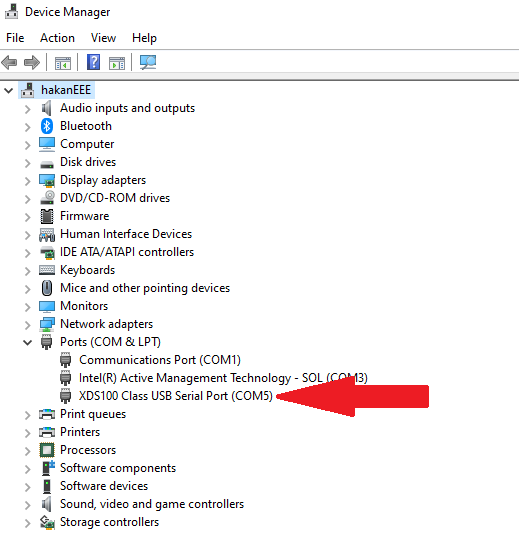
\includegraphics[scale=0.5]{Figures/DeviceManager.png}
	\caption{The serial port on the Device Manager screen}
	\label{fig:DeviceManager}
\end{figure}



\section{\href{https://github.com/hakansrc/fault_tolerant_drives/tree/master/Software/MultipleDataPlot/MultipleFloatDataSender}{MultipleFloatDataSender library}}
This library is the critical part of the EEVL. For the embedded environment, all the necessary functions and/or variables are defined in this library. In order to add the library to a CCS project, there are three steps to be done.
\subsection{Adding library to a CCS project}
\label{subsection:addinglibrary}
\begin{enumerate}
	\item Add the \href{https://github.com/hakansrc/fault_tolerant_drives/blob/master/Software/MultipleDataPlot/MultipleFloatDataSender/Debug/MultipleFloatDataSender.lib}{MultipleFloatDataSender.lib} file to \textbf{Build} -> \textbf{C2000 Linker} -> \textbf{File Search Path}, as shown in Figure \ref{fig:dotlibfile}.
	\item Add the library project path to the included path, as show in Figure \ref{fig:libraryincludepath}
	\item Include the library header \textbf{"MultipleFloatDataSender.h"} to the project, as shown in Figure \ref{fig:includeheader}
\end{enumerate}
\begin{figure}[H]
	\centering
	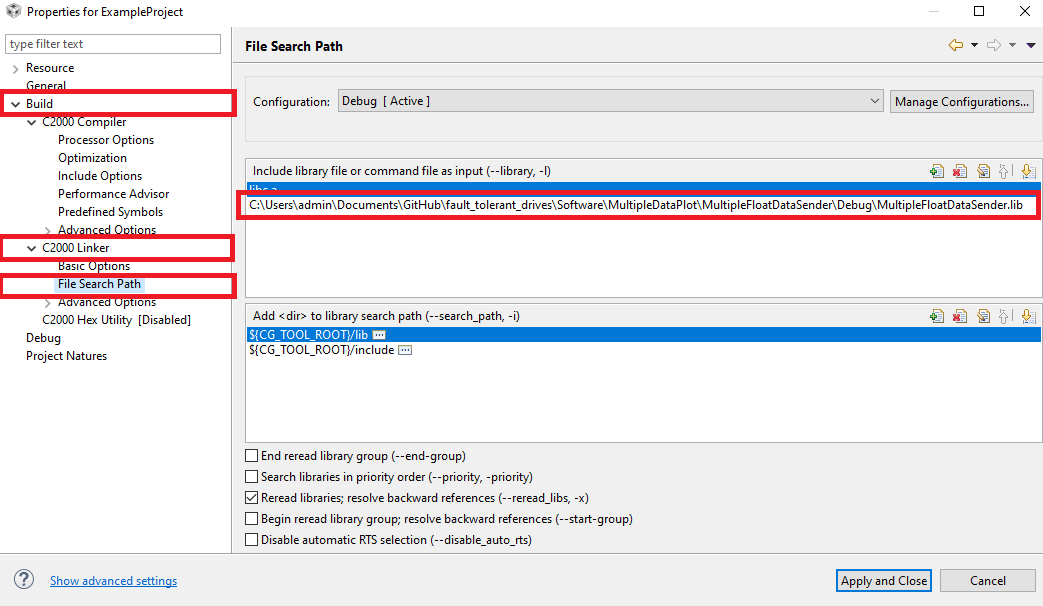
\includegraphics[scale=0.5]{Figures/dotlibfile.png}
	\caption{Linking the library file}
	\label{fig:dotlibfile}
\end{figure}

\begin{figure}[H]
	\centering
	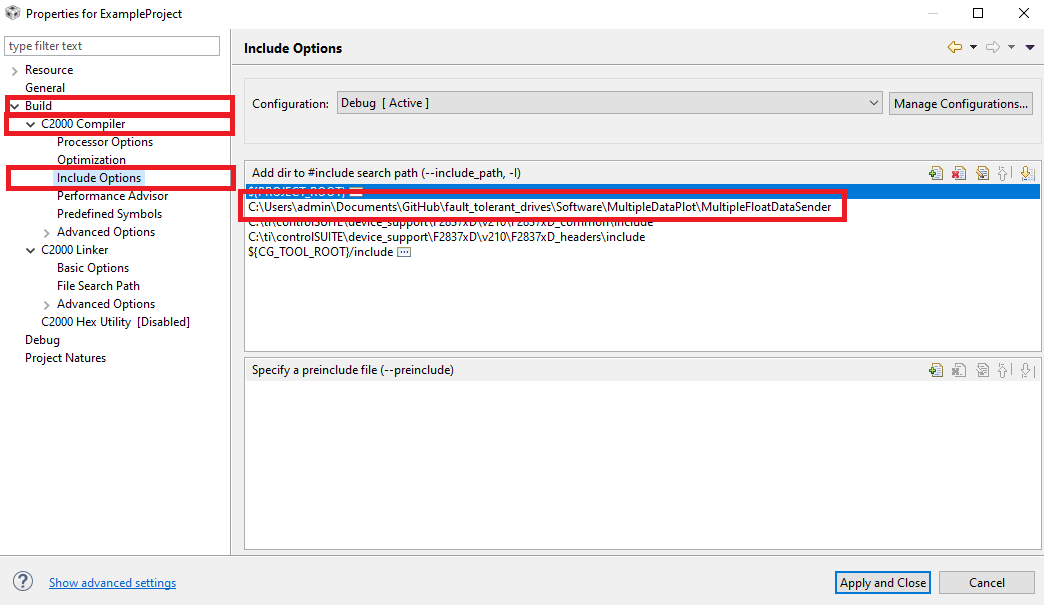
\includegraphics[scale=0.5]{Figures/libraryincludepath.png}
	\caption{Addition of library path to the project}
	\label{fig:libraryincludepath}
\end{figure}
\begin{figure}[H]
	\centering
	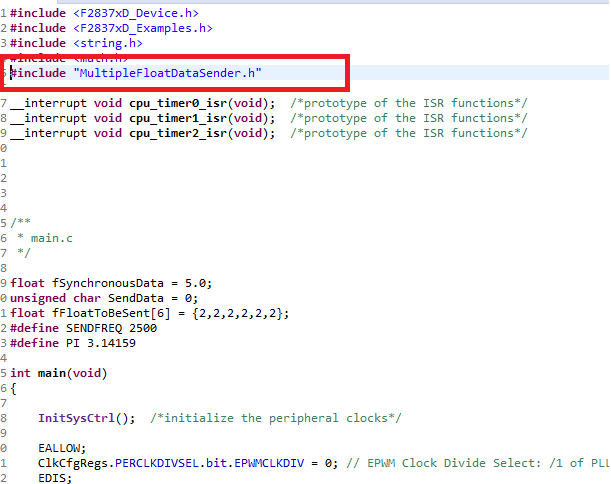
\includegraphics[scale=0.5]{Figures/includeheader.png}
	\caption{Addition of library path to the project}
	\label{fig:includeheader}
\end{figure}

\subsection{The content of the MultipleFloatDataSender library}
For initializations and operation, the library has several functions. Each of these functions and an example usage is provided in this section
\subsubsection{void InitializeSciaRegisters(float fSciBaudRate)}
\label{subsubsection:InitializeSciaRegisters}
\begin{addmargin}[4em]{1em}
	\paragraph{Description}
	InitializeSciaRegisters() attempts to initialize the Scia registers for the library operation. The baudrate of the channel can be set by the \textbf{fSciBaudRate} variable. 
	
	The GPIOs for the Scia are \textbf{\underline{NOT}} initialized. The developer should initliaze the preferred Scia GPIOs by him/herself.



	\paragraph{Return value}
	This function has no return value.
	\paragraph{Cautions}
	\label{subsubsubsubsection:caution-InitializeSciaRegisters}
	This function does not initialize the GPIOs for SCIA. The user must initialize the GPIOs by him/herself.

	For \textbf{F28379D LaunchPad}, GPIO42 and GPIO43 must be set to Scia module. For \textbf{F28379D controlCARD}, GPIO28 and GPIO29 must be set to Scia module. If you are using some external JTAG probe, the scia GPIOs that are connected to the FTDI chip must be initialized.
\end{addmargin}
\subsubsection{void SciaBackgroundTask(void)}
\label{subsubsection:sciabackgroundtask}
\begin{addmargin}[4em]{1em}
	\paragraph{Description}
	SciaBackgroundTask() governs the sending of the data through SCI interface. To be able to send the data packets through SCI, this function should be called periodically. It is advised to call this function outside of ISRs. 
	\paragraph{Return value}
	This function has no return value.
	\paragraph{Cautions}
	This function should be called  \textbf{\underline{at least}} once every 1 milisecond, can be called more frequent as well. It is advised to call this function outside of the ISRs. An example call is given in \href{https://github.com/hakansrc/fault_tolerant_drives/blob/master/Software/MultipleDataPlot/ExampleProject/main.c}{\underline{\textbf{this link}}}.
\end{addmargin}
\subsubsection{int SciSendMultipleFloatWithTheTag(float *FloatArrayToBeSent, uint16\_t ui16NumberOfFloats)}
\label{subsubsection:scisendmultiplefloat}
\begin{addmargin}[4em]{1em}
	\paragraph{Description}
	SciSendMultipleFloatWithTheTag() is the function that is used for sending the data to the computer. 
	
	When called, this function sends \textbf{ui16NumberOfFloats} number of floats inside the \textbf{FloatArrayToBeSent} array. An example usage of this function can be found in \href{https://github.com/hakansrc/fault_tolerant_drives/blob/master/Software/MultipleDataPlot/ExampleProject/main.c}{\underline{\textbf{this link}}}.
	\paragraph{Return value}
	On success, this function returns the number of bytes that is sent through Scia. 
	This function return -1 if the data buffer of the Scia is full.
	\paragraph{Cautions}
	To send 6 float numbers with 921600 baudrate value, the maximum call rate of the function should not exceed 3kHz. 
	
	The reason is that a package of data consists of 4 bytes of tag data and 4 bytes for each float number, therefore each data package consists of 28 bytes. To send 28 bytes of data, 280 bits are sent through the Scia (8 bit data, 1 start bit, 1 stop bit). All these values results in the maximum data rate stated in (\ref{eqn:datarate}).

	\begin{equation} \label{eqn:datarate}
		Maximum Package Rate  = \frac{Baud Rate Value(bits/sec)}{Bits Per Package} = \frac{921600}{280}= 3300  \:\: \mathrm{packages/sec}
	\end{equation}
\end{addmargin}

\subsubsection{int SciaUartSend\_NoInterrupt(char *BuffWriteArray, unsigned int lengthOfData);}
\begin{addmargin}[4em]{1em}
	\paragraph{Description}
	This function sends \textbf{lengthOfData} bytes of data starting from the address stated with \textbf{BuffWriteArray} pointer. 

	For the normal operation of the MultipleFloatDataSender library, SciaUartSend\_NoInterrupt function is not used. 

	\paragraph{Return value}
	On success, this function returns the number of bytes that is sent through Scia. 
	\paragraph{Cautions}
	For the normal operation of the MultipleFloatDataSender library, SciaUartSend\_NoInterrupt function is not used. 

\end{addmargin}

\section{Using the EEVL library}
Before starting to use the EEVL library make sure that the followings are done.
\begin{enumerate}
	\item The options of \href{https://github.com/hakansrc/fault_tolerant_drives/blob/master/Software/MultipleDataPlot/DataReceiver.m}{DataReceiver.m} (stated in \ref{subsubsection:Options}) has been properly set.
	\item The \href{https://github.com/hakansrc/fault_tolerant_drives/tree/master/Software/MultipleDataPlot/MultipleFloatDataSender}{MultipleFloatDataSender library} should be initialized properly, as explained in \ref{subsection:addinglibrary}.
	\item The corresponding gpios of the Scia must be initialized. For \textbf{F28379D LaunchPad}, GPIO42 and GPIO43 must be set to Scia module. For \textbf{F28379D controlCARD}, GPIO28 and GPIO29 must be set to Scia module. 
	\item Scia registers are initialzed properly, as explained in \ref{subsubsection:InitializeSciaRegisters}
	\item SciaBackgroundTask is called at least 1kHz rate, as stated in \ref{subsubsection:sciabackgroundtask}
	\item SciSendMultipleFloatWithTheTag function is called at a rate of 3kHz (max), as stated in \ref{subsubsection:scisendmultiplefloat}.
\end{enumerate}

Overall, \href{https://github.com/hakansrc/fault_tolerant_drives/tree/master/Software/MultipleDataPlot/ExampleProject}{\color{blue}{\underline{an example CCS project}}} and recommended settings for the \href{https://github.com/hakansrc/fault_tolerant_drives/blob/master/Software/MultipleDataPlot/DataReceiver.m}{\color{blue}{\underline{DataReceiver.m}}} are provided as hyperlinks.

\section{Bugs and Warnings}
\begin{enumerate}
	\item During operation \href{https://github.com/hakansrc/fault_tolerant_drives/blob/master/Software/MultipleDataPlot/DataReceiver.m}{DataReceiver.m} might give deficient data error as shown in Figure \ref{fig:deficientdataerror}. If you get this error too much (around once a second) it is recommended to reduce the value of \textbf{ProcessRawDataThresholdInBytes} inside the \href{https://github.com/hakansrc/fault_tolerant_drives/blob/master/Software/MultipleDataPlot/DataReceiver.m}{DataReceiver.m} routine. 
	\item If the serial channel has already been opened, you might get the error given in Figure \ref{fig:alreadyopenerror}. You should call "fclose(instrfind)" command in MATLAB to close, if the device is opened with MATLAB and not closed. (If the device opened by some other program, then that program must be closed.)
\end{enumerate}

\begin{figure}[H]
	\centering
	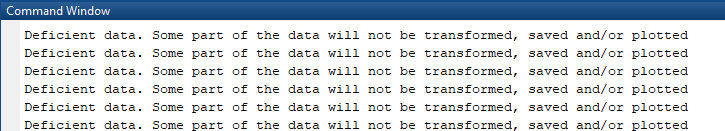
\includegraphics[scale=0.5]{Figures/deficientdataerror.PNG}
	\caption{Deficient data error}
	\label{fig:deficientdataerror}
\end{figure}
\begin{figure}[H]
	\centering
	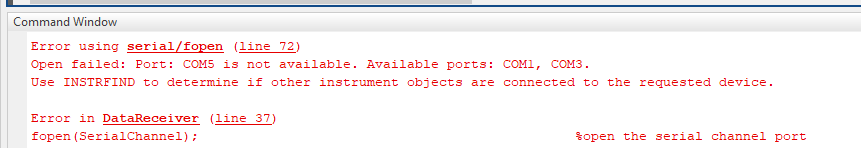
\includegraphics[scale=0.5]{Figures/alreadyopen.PNG}
	\caption{The serial channel device already open error}
	\label{fig:alreadyopenerror}
\end{figure}


\bibliographystyle{plain}
\bibliography{references}
\end{document}
